\documentclass[polish,envcountsect,10pt]{beamer}
    \usepackage[T1]{fontenc}
    \usepackage{listings}
    \usepackage{fontspec}                 % żeby ustawić czcionkę na systemową (Arial)
    \usepackage[utf8x]{inputenc}
    \usepackage{polski}
    \usepackage{multicol}
    \usepackage{babel}
    \usepackage{hyperref}
    \usepackage{graphicx}
    \usepackage{outlines}
    \usepackage{algorithm2e}
    \usepackage{tikz}

    \newtheorem{mdfn}{Definicja}
    \newtheorem{twrdz}{Twierdzenie}
    \newtheorem{lmt}{Lemat}


    \usetheme{Frankfurt}

    \title{Rozwiązywanie gier}
    \author{Michał Krakowiak}
    \subtitle{Wybrane problemy algorytmiczne i technologiczne, seminarium}
    \date{Gdańsk, 05.11.2019}
    
\begin{document}
    \frame{\titlepage}
    \section{Wstęp}
        \subsection{Zawartość}
            \begin{frame}
                \frametitle{Zawartość}
                \begin{multicols}{2}
                    \tableofcontents[pausesections]                    
                \end{multicols}
            \end{frame}
        \subsection{Tło historyczne}
            \begin{frame}
                \frametitle{Tło historyczne}
                \begin{columns}
                    \column{0.5\textwidth}
                        \begin{figure}[H]
                            \centering
                                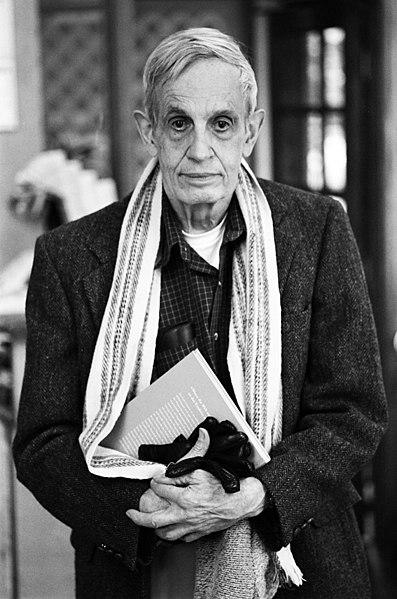
\includegraphics[width=0.7\textwidth]{images/nash.jpg}
                            \caption{John Nash}
                        \end{figure}
                    \column{0.5\textwidth}
                    \begin{figure}[H]
                        \centering
                            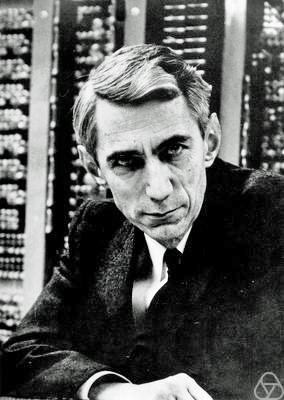
\includegraphics[width=0.7\textwidth]{images/shannon.jpg}
                        \caption{Claude Shannon}
                    \end{figure}
                \end{columns}
            \end{frame}
        \subsection{Definicja gry}
            \begin{frame}
                \frametitle{Czym jest gra?}
                    \begin{mdfn}
                        Gra jest opisem strategicznej interakcji, która narzuca ograniczenia na udział graczy oraz akcje jakie mogą podjąć \cite{course_gt}.
                        %A game is a description of strategic interaction that includes the constraints on the actions that the players can take and the players’ interests, but does not specify the actions that the players do take. A solution is a systematic description of the outcomes that may emerge in a family of games. Game theory suggests reasonable solutions for classes of games and examines their properties.
                    \end{mdfn}
            \end{frame}
            \begin{frame}
                \frametitle{Gra w ujęciu kombinatorycznym}
                Właściwości rozważanych gier:
                \begin{itemize}
                    \item<2-> Udział tylko dwóch graczy
                    \item<3-> Gracze wykonują ruchy naprzemiennie
                    \item<4-> Przebieg nie zależy od czynników losowych
                    \item<5-> Gracze posiadają pełną wiedzę o stanie gry
                    \item<6-> Gra kończy się po skończonej liczbie ruchów
                    \item<7-> Wygrywa gracz, który wykona ostatni ruch
                \end{itemize}
            \end{frame}
    \section{Klasyfikacja rozwiązań}
        \subsection{Przegląd}
            \begin{frame}
                \frametitle{Klasyfikacja rozwiązań}
                \begin{itemize}
                    \item<1-> Mocne
                    \item<2-> Słabe
                    \item<3-> Ultra słabe
                \end{itemize}
            \end{frame}
        \subsection{Mocne}
            \begin{frame}
                \frametitle{Rozwiązania mocne}
                \begin{itemize}
                    \item<1-> Jest znany algorytm pozwalający uzyskać optymalne ruchy z każdej pozycji (nawet jeżeli, któryś z graczy popełnił błąd)
                    \item<2-> Częste wykorzystanie metod siłowych
                    \item<3-> Dowód może nie być pomocny w zrozumieniu powodów dlaczego dana gra jest rozwiązywalna
                \end{itemize}
            \end{frame}
            \subsubsection{Kółko i krzyżyk}
                \begin{frame}
                    \frametitle{Kółko i krzyżyk}
                    \begin{columns}
                        \column{0.6\textwidth}
                            \begin{itemize}
                                \item<1-> Gra jest trywialna, ze względu na niewielkie drzewo gry
                                \item<2-> Teoretyczna liczba stanów to $3^9 = 19683$
                                \item<3-> Nie każdy stan jest możliwy
                                \item<4-> Niektóre stany są tożsame
                                \item<7-> W rezultacie jest tylko $765$ różnych stanów \cite{tictactoe}
                            \end{itemize}
                        \column{0.4\textwidth}
                            \only<1-2>{
                                \begin{figure}[H]
                                    \centering
                                    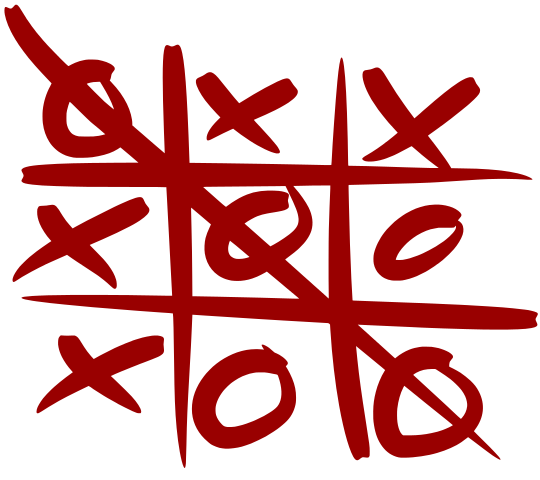
\includegraphics[width=\textwidth,natwidth=540,natheight=480]{images/Tic_tac_toe.svg.png}
                                    \caption{Kółko i krzyżyk}
                                \end{figure}
                            }
                            \only<3->{
                                \begin{table}
                                    \center
                                \begin{tabular}{| c | c | c |}
                                    \hline X & X & X \\
                                    \hline O & O & O \\
                                    \hline   &   &   \\
                                    \hline
                                \end{tabular}
                            \end{table}
                            }
                            \only<4->{
                                \begin{table}
                                    \center
                                \begin{tabular}{| c | c | c |}
                                    \hline   &   &   \\
                                    \hline   &   & O \\
                                    \hline X & X & O \\
                                    \hline
                                \end{tabular}
                            \end{table}
                            }
                            \only<5->{
                            \begin{table}
                                \begin{tabular}{| c | c | c |}
                                    \hline X & X & O \\
                                    \hline   &   & O \\
                                    \hline   &   &   \\
                                    \hline
                                \end{tabular}
                            \end{table}
                            }
                            \only<6->{
                            \begin{table}
                                \begin{tabular}{| c | c | c |}
                                    \hline O & X & X \\
                                    \hline O &  &   \\
                                    \hline   &   &   \\
                                    \hline
                                \end{tabular}
                            \end{table}
                            }
                    \end{columns}
                \end{frame}
                \begin{frame}
                    \frametitle{Kółko i krzyżyk}
                    \begin{columns}
                        \column{0.5\textwidth}
                        \begin{figure}[H]
                            \centering
                            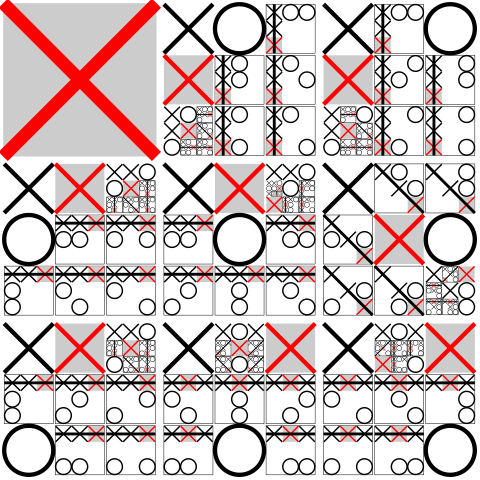
\includegraphics[width=\textwidth,natwidth=480,natheight=480]{images/480px-Tictactoe-X.svg.png}
                            \caption{Optymalna gra dla X}
                        \end{figure}
                        \column{0.5\textwidth}
                        \begin{figure}[H]
                            \centering
                            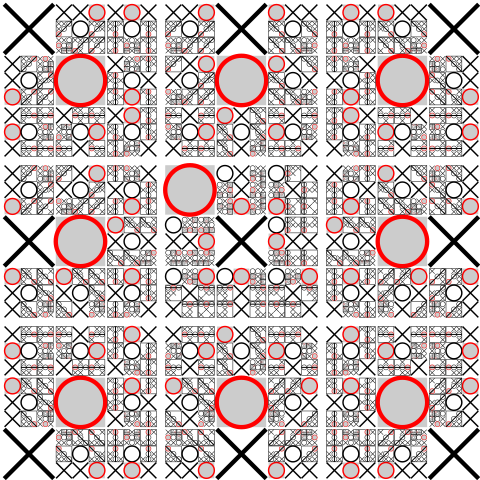
\includegraphics[width=\textwidth,natwidth=480,natheight=480]{images/480px-Tictactoe-O.svg.png}
                            \caption{Optymalna gra dla O}
                        \end{figure}
                    \end{columns}
                \end{frame}
            \subsubsection{Nim}
                \begin{frame}
                    \frametitle{Nim}
                    \begin{columns}
                        \column{0.6\textwidth} 
                        \begin{itemize}
                            \item<1-> Matematyczna gra strategiczna
                            \item<2-> Gracze zabierają elementy ze stosów
                            \item<3-> W czasie ruchu gracz bierze dowolną niezerową liczbę elementów
                            \item<4-> W jednym ruchu można zabrać elementy z tylko jednego stosu
                            \item<5-> W klasycznej wersji wygrywa gracz, który zabierze ostatni element
                        \end{itemize}
                        \column{0.4\textwidth}
                        \begin{figure}[H]
                            \centering
                            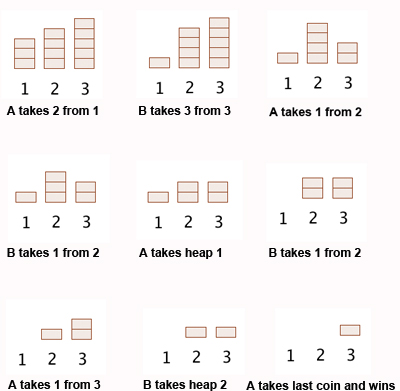
\includegraphics[width=\textwidth]{images/nim_game}
                            \caption{Przykładowa rozgrywka w nim}
                        \end{figure}
                    \end{columns}
                \end{frame}
                \begin{frame}
                    \frametitle{Nim - strategia}
                        \begin{itemize}
                            \item<1->Kombinatoryczna teoria gier definiuje działanie tzw. \textit{nimsumy}: $x \oplus y$
                            \item<2-> Działanie jest także znane jako \textit{alternatywa wykluczająca}, czyli xor
                            \item<3-> $(a \oplus b) \oplus c = a \oplus (b \oplus c)$
                            \item<4-> $a \oplus b = b \oplus a$
                            \item<5-> $0 \oplus a = a$
                            \item<6-> $a \oplus a = 0$
                        \end{itemize}
                \end{frame}
                \begin{frame}
                    \frametitle{Nim - strategia}
                        \begin{twrdz}
                            Gracz rozpoczynający ma wygrywającą strategię wtedy i tylko wtedy, gdy nimsuma rozmiarów stosów jest niezerowa. W przeciwnym razie drugi gracz posiada strategię wygrywającą.
                        \end{twrdz} 
                \end{frame}
                \begin{frame}
                    \frametitle{Nim - strategia}
                        \begin{itemize}
                            \item<1-> $x_i$ - ilość elementów przed wykonaniem ruchu na $i$-tym stosie
                            \item<2-> $y_i$ - ilość elementów po wykonaniu ruchu na $i$-tym stosie
                            \item<3-> Niech $s = x_1 \oplus ... \oplus x_n$
                            \item<4-> Niech $t = y_1 \oplus ... \oplus y_n$
                            \item<5-> $t = 0 \oplus t $ 
                            \item<6-> $t = (s \oplus s) \oplus t$
                            \item<7-> $t = s \oplus (s \oplus t)$
                            \item<8-> $t = s \oplus (x_1 \oplus ... \oplus x_n) \oplus (y_1 \oplus ... \oplus y_n)$
                            \item<9-> $t = s \oplus (x_1 \oplus y_1) \oplus ... \oplus (x_n \oplus y_n) $
                            \item<10-> $t = s \oplus 0 \oplus ... \oplus 0 \oplus (x_k \oplus y_n) \oplus 0 \oplus ... \oplus 0$
                            \item<11-> $t = s \oplus x_k \oplus y_k$
                        \end{itemize}
                \end{frame}
                \begin{frame}
                    \frametitle{Nim - strategia}
                    \begin{columns}
                        \column{0.6\textwidth}
                            \begin{itemize}
                                \item<1-> $x_i$ - ilość elementów przed wykonaniem ruchu na $i$-tym stosie
                                \item<1-> $y_i$ - ilość elementów po wykonaniu ruchu na $i$-tym stosie
                                \item<1-> Niech $s = x_1 \oplus ... \oplus x_n$
                                \item<1-> Niech $t = y_1 \oplus ... \oplus y_n$
                                \item<1-> $t = s \oplus x_k \oplus y_k$
                                \item<2-> Jeżeli $s = 0,$ gracz wykonujący ruch przegrywa
                                \item<3-> Jeżeli nie ma już możliwych ruchów, gra się skończyła i gracz już przegrał
                                \item<4-> Każdy możliwy ruch sprawia, że $t = x_k \oplus y_k \neq 0$
                                \item<5-> $x_k \oplus y_k \neq 0$, ponieważ gracz musi pobrać niezerową liczbę elementów
                            \end{itemize}
                        \column{0.4\textwidth}
                        \begin{figure}[H]
                            \centering
                            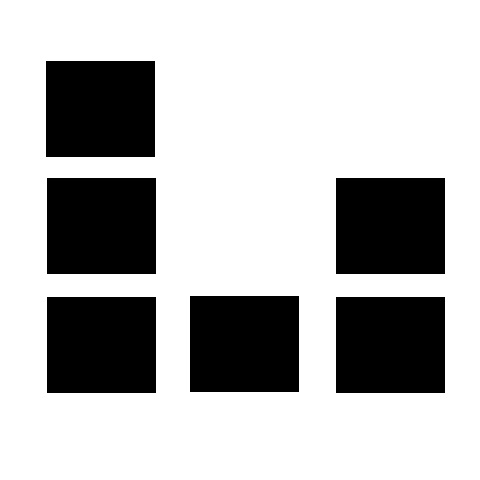
\includegraphics[width=\textwidth]{images/nimsuma0.jpg}                            
                        \end{figure}
                    \end{columns}
                \end{frame}
                \begin{frame}
                    \frametitle{Nim - strategia}
                    \begin{columns}
                        \column{0.6\textwidth}
                            \begin{itemize}
                                \item<1-> $x_i$ - ilość elementów przed wykonaniem ruchu na $i$-tym stosie
                                \item<1-> $y_i$ - ilość elementów po wykonaniu ruchu na $i$-tym stosie
                                \item<1-> Niech $s = x_1 \oplus ... \oplus x_n$
                                \item<1-> Niech $t = y_1 \oplus ... \oplus y_n$
                                \item<1-> $t = s \oplus x_k \oplus y_k$
                                \item<2-> Jeżeli $s \neq 0,$ to możliwe jest wykonanie takiego ruchu, że $t = 0$, gracz wykonujący ruch wygrywa
                                \item<3-> Żeby $t = 0$, to $y_k = s \oplus x_k$
                                \item<4-> $t = s \oplus x_k \oplus (s \oplus x_k) = 0$
                            \end{itemize}
                    \column{0.4\textwidth}
                        \begin{figure}[H]
                            \centering
                            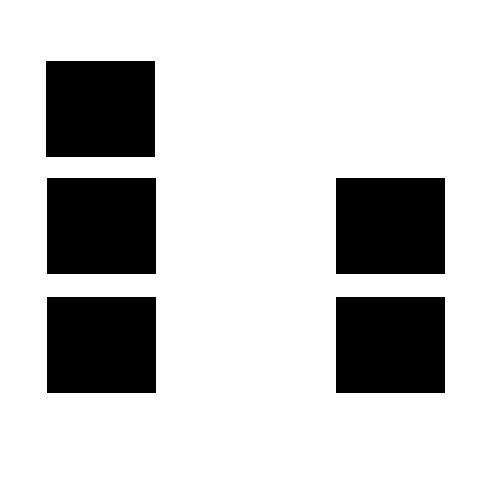
\includegraphics[width=\textwidth]{images/nimsuma1.jpg}                            
                        \end{figure}
                \end{columns}
                 
                \end{frame}
                \begin{frame}
                    \frametitle{Nim - strategia}
                    \begin{itemize}
                        \item<1-> $x_i$ - ilość elementów przed wykonaniem ruchu na $i$-tym stosie
                        \item<1-> $y_i$ - ilość elementów po wykonaniu ruchu na $i$-tym stosie
                        \item<1-> Niech $s = x_1 \oplus ... \oplus x_n$
                        \item<1-> Niech $t = y_1 \oplus ... \oplus y_n$
                        \item<2-> Strategia wygrywająca polega na zdejmowaniu elementów w taki sposób, aby zaszło $t = 0$
                        \item<3-> Taki ruch jest możliwy wtedy i tylko wtedy, gdy $s \neq 0$ \pause $\qed$
                    \end{itemize}
                \end{frame}
        %\subsubsection{Zgadnij kto to?}
        %    \begin{frame}
        %        \frametitle{Zgadnij kto to?}
        %    \end{frame}
            \subsection{Słabe}
            \begin{frame}
                \frametitle{Rozwiązania słabe}
                \begin{itemize}
                    \item<1-> Jest znany algorytm, który pozwala jednemu z graczy utrzymać zwycięstwo lub remis od początku gry, niezależnie od ruchów przeciwnika
                    \item<2-> Dzięki podanemu algorytmowi uzyskano przynajmniej jedną \textit{optymalną grę} oraz podano dowód, że każdy ruch jest optymalny dla gracza, który go wykonuje                    
                \end{itemize}     
            \end{frame}
            \subsubsection{Warcaby}
                \begin{frame}
                    \frametitle{Warcaby}
                    \begin{columns}
                        \column{0.6\textwidth}
                        \begin{itemize}
                            \item<1-> Chinook - program komputerowy rozwijany w latach 1989 - 2007
                            \item<2-> 19.07.2007 w magazynie \textit{Science} twórcy opublikowali swój dowód, że w przypadku, gdy żaden z graczy nie popełni błędu partia kończy się remisem
                            \item<3-> Baza danych końcówek o liczbie pionów $\leq 10$, \textbf{237 GB}
                            \item<4-> Baza danych przechowuje wynik gry dla danej pozycji, jest wykorzystywana do analizy wstecz (retrograde)
                            \item<4-> Drugi komponent: algorytm przeszukiwania wprzód (alphabeta)
                        \end{itemize}
                        \column{0.4\textwidth}
                        \begin{figure}[H]
                            \centering
                            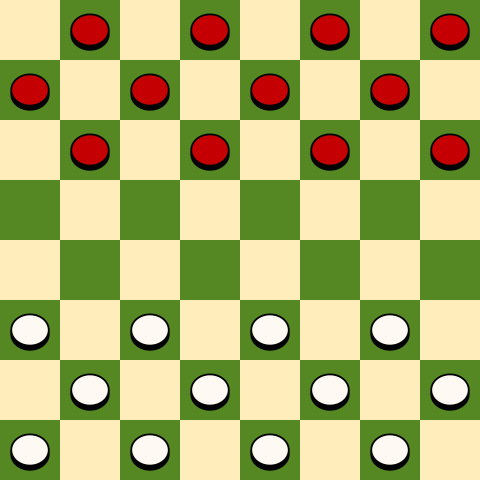
\includegraphics[width=\textwidth]{images/checkers}
                            \caption{Warcaby}
                        \end{figure}
                    \end{columns}
                \end{frame}
            \subsubsection{Szachy Gardnera 5x5}
                \begin{frame}
                    \frametitle{Szachy Gardnera 5x5}
                    % https://chess.stackexchange.com/questions/24042/studying-why-gardners-minichess-variant-is-solved
                    \begin{columns}
                        \column{0.6\textwidth}
                        \begin{itemize}
                            \item Udowodniono remis, przy optymalnej grze obu graczy \cite{minichess}
                        \end{itemize}
                        \column{0.4\textwidth}
                            \begin{figure}[H]
                                \centering
                                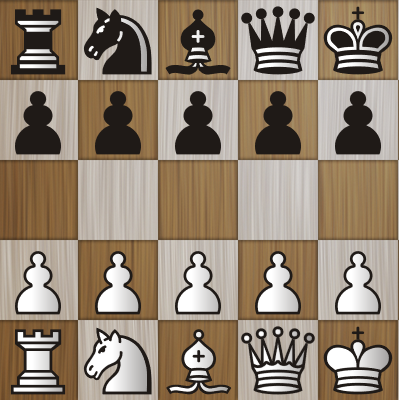
\includegraphics[width=\textwidth]{images/gardner.png}
                                \caption{Startowe ułożenie w szachach Gardnera 5x5}
                            \end{figure}    
                    \end{columns}
                \end{frame}
                \begin{frame}
                    \frametitle{Szachy Gardnera 5x5}
                    % https://chess.stackexchange.com/questions/24042/studying-why-gardners-minichess-variant-is-solved
                            \begin{figure}[H]
                                \centering
                                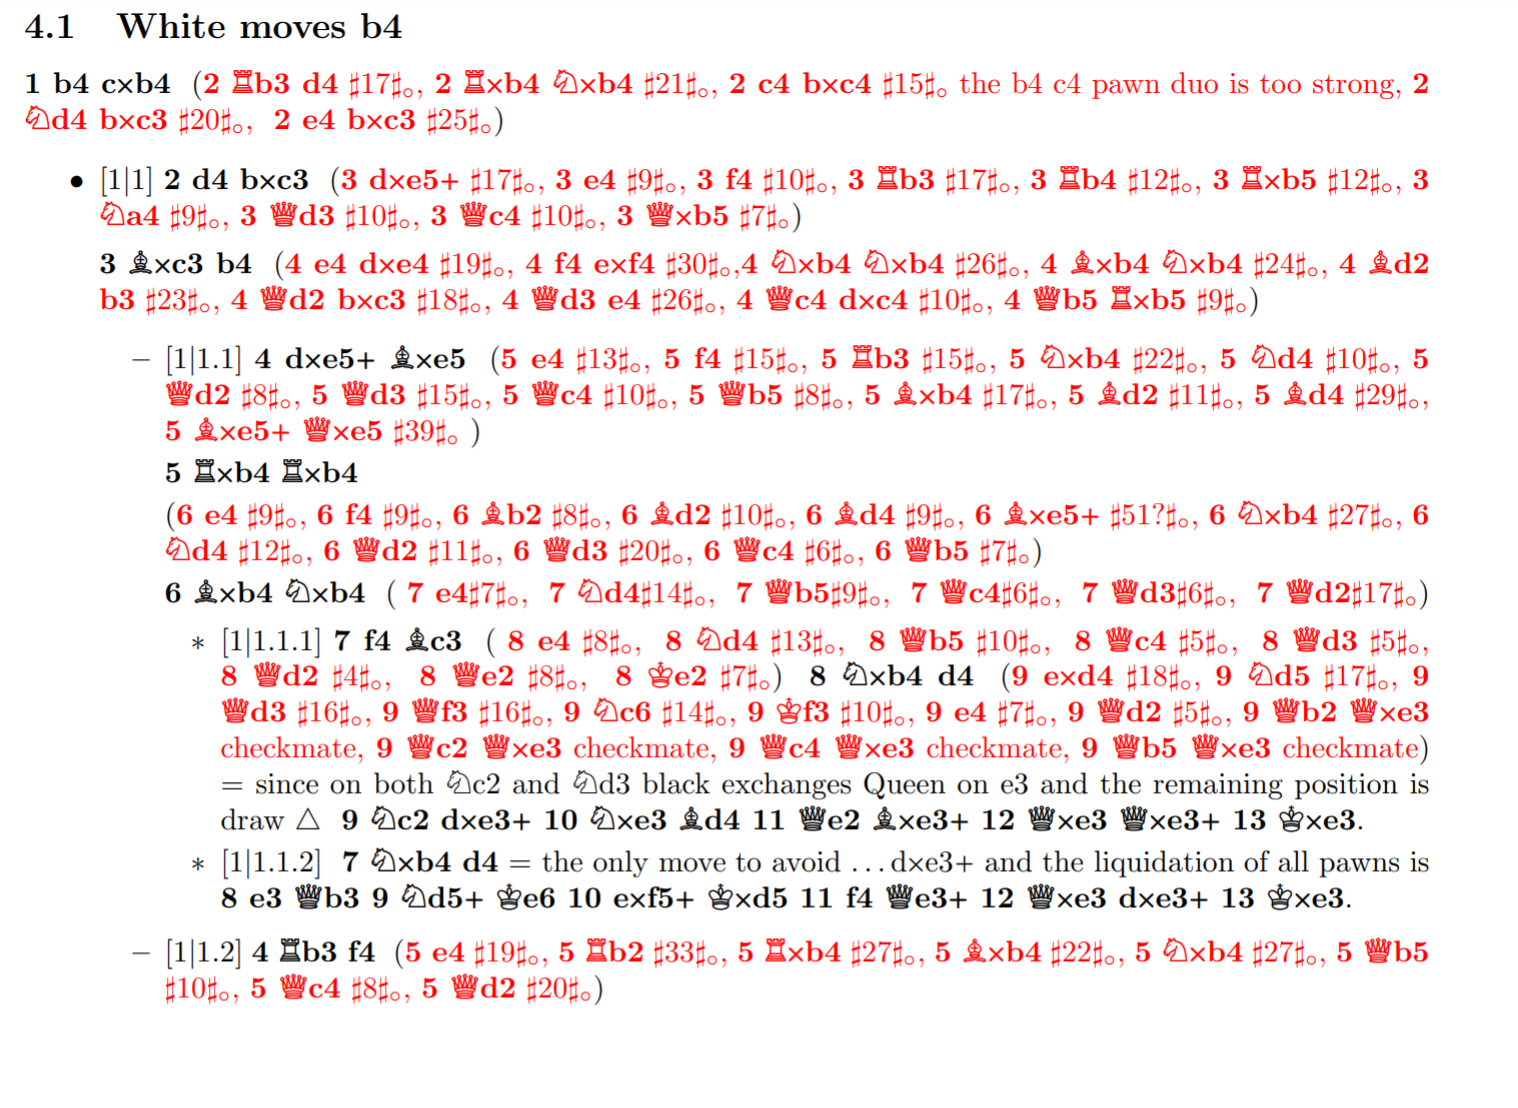
\includegraphics[width=0.8\textwidth]{images/gardner_proof}
                                \caption{Fragment rozwiązania szachów 5x5}
                            \end{figure}    
                \end{frame}

        \subsection{Ultra słabe}
            \begin{frame}
                \frametitle{Rozwiązania ultra słabe}
                \begin{itemize}
                    \item<1-> Udowodniono, że gracz wygrywa/przegrywa/remisuje ze startowej pozycji, jeżeli wszyscy grają optymalnie
                    \item<2-> Przeprowadzony dowód może być niekonstruktywny
                    \item<3-> \textbf{Nie jest wymagane określenie żadnego z ruchów optymalnej gry}
                    % go,
                    %kradziez strategii
                \end{itemize}
            \end{frame}
            \subsubsection{Hex}
                \begin{frame}
                    \frametitle{Hex}
                    \begin{columns}
                        \column{0.6\textwidth}
                            \begin{itemize}
                                \item<1-> Tradycyjnie rozgrywana na planszy w kształcie rombu 11x11
                                \item<2-> Gracze dysponują kamieniami o odmiennych kolorach
                                \item<3-> Gracze układają kamienie na wolnych polach
                                \item<4-> Wygrywa ten, który utworzy nieprzerwany ciąg łączący boki planszy własnego koloru
                            \end{itemize}
                        \column{0.4\textwidth}
                        \begin{figure}[H]
                            \centering
                            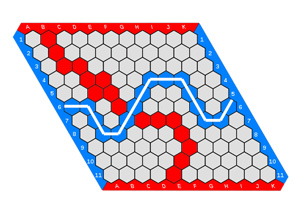
\includegraphics[width=\textwidth]{images/hex}
                            \caption{Rozgrywka w hex}
                        \end{figure}
                    \end{columns}                    
                \end{frame}
                \begin{frame}
                    \frametitle{Hex - Dowód Johna Nasha}
                    \begin{twrdz}
                        Pierwszy gracz ma strategię wygrywającą
                    \end{twrdz}
                    \begin{lmt}
                        Dodatkowy lub losowy element Twojego koloru nie może Ci zaszkodzić
                    \end{lmt} \pause
                    \begin{lmt}
                        Hex nie może zakończyć się remisem
                    \end{lmt} \pause
                    \begin{proof}
                        Mamy dwóch graczy A i B, A zaczyna. Załóżmy, że B ma strategię wygrywającą. A może zagrać w losowe miejsce. Teraz A jest efektywnym drugim graczem i może grać strategią wygrywającą \cite{hex_proof}.
                    \end{proof}
                \end{frame}
                \begin{frame}
                    \frametitle{Hex - Dowód Johna Nasha}
                    Przedstawiony dowód korzystający z kradzieży strategii, może być zastosowany do każdej symetrycznej gry, w której posiadanie dodatkowego elementu na planszy (lub dodatkowego ruchu) nie szkodzi danemu graczowi.
                \end{frame} 
            \subsubsection{Go}
                \begin{frame}
                    \frametitle{Go}
                    \begin{columns}
                        \column{0.6\textwidth}
                            \begin{itemize}
                                \item<1-> Tylko wersja gry bez komi
                                \item<2-> Komi to wyrównanie punktowe dla drugiego gracza
                                \item<3-> Dowód korzysta z kradzieży strategii
                                \item<4-> W Go można pasować
                                \item<5-> Jeżeli białe mają strategię wygrywającą, czarne mogą ją ukraść pasując już na początku gry
                                \item<6-> W rezultacie czarne mogą wygrać lub zremisować przy optymalnej grze
                            \end{itemize}
                        \column{0.4\textwidth}
                            \begin{figure}[H]
                                \centering
                                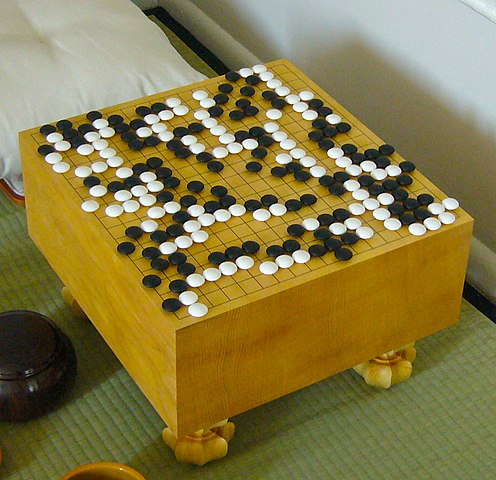
\includegraphics[width=\textwidth]{images/496px-FloorGoban.jpg}
                                \caption{Goban}
                            \end{figure} 
                    \end{columns}                    
                \end{frame}
            
    \section{Szachy}
        \begin{frame}
            \frametitle{Szachy}
            \begin{columns}
            \column{0.6\textwidth}                
            \begin{itemize}
                \item<1-> $10^{120}$ możliwych wariantów
                \item<2-> Rozwiązane częściowo
                \item<3-> Znane są rozwiązania mocne dla wszystkich końcówek liczących od 3 do 7 bierek (wliczając obu króli)
                \item<4-> Osiągnięto to dzięki bazie danych końcówek i analizie retrograde
           \end{itemize}
            \column{0.4\textwidth}                
            \begin{figure}[H]
                \centering
                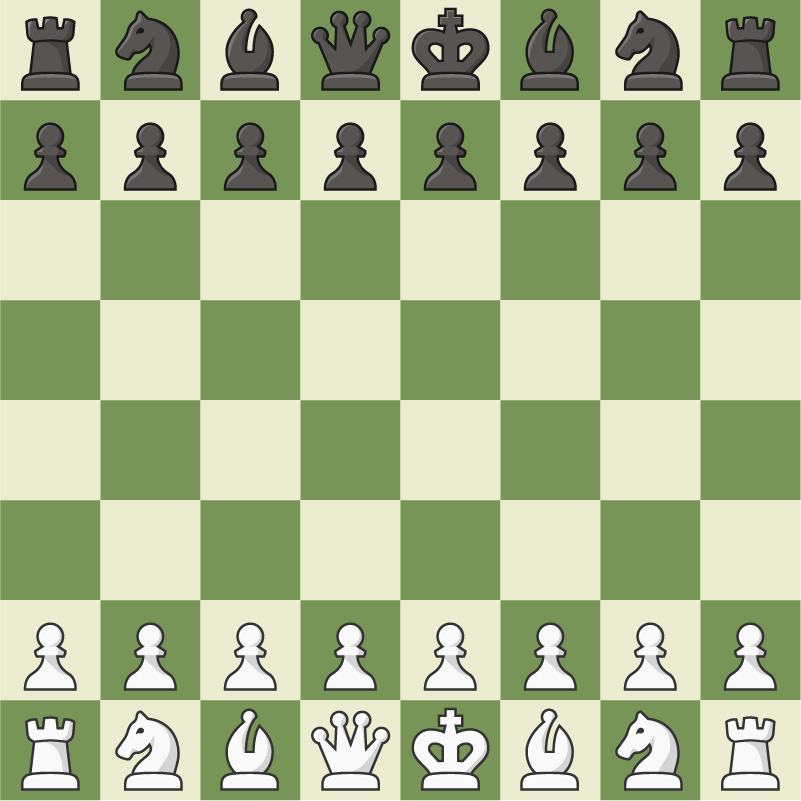
\includegraphics[width=\textwidth]{images/chess.png}
                \caption{Szachy klasyczne}
            \end{figure}
            %podzial na otwarcie, gra srodkowa, koncowki
            %retro grade
        \end{columns}
        \end{frame}
        \subsection{Minimax}
            \begin{frame}
                \frametitle{Minimiax}
                \begin{figure}[H]
                    \centering
                    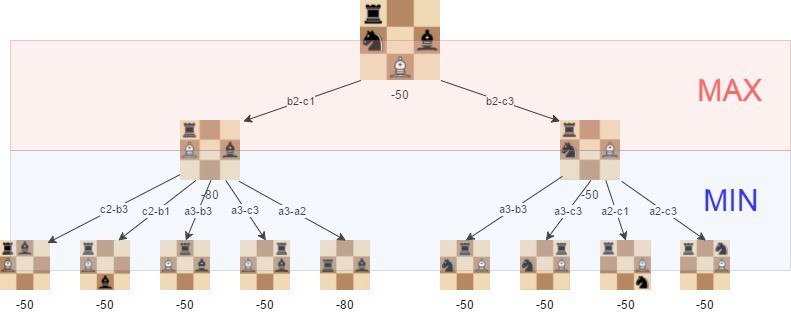
\includegraphics[width=\textwidth]{images/minimax}
                    \caption{Przykładowy minimax}
                \end{figure}
            \end{frame}
            \begin{frame}
                \frametitle{Minimax}
                \scalebox{0.85}{
                            \begin{minipage}{1.1\linewidth}
                \begin{algorithm}[H]
                    \SetAlgoLined
                    \DontPrintSemicolon
                    \SetKwFunction{FMain}{minimax}
                    \SetKwProg{Fn}{Function}{:}{end}
                    \Fn{\FMain{node, depth, maximizingPlayer}}{
                        \If{depth $=0$ or node is a terminal node}
                        {
                            \KwRet heuristic value of node\;
                        }
                        \eIf{maximizingPlayer}
                        {
                            value $\gets -\infty$\;
                            \ForEach{child in node}{
                                value $\gets$ max(value, minimax(child, depth $- 1$, False))\;
                            }
                            \KwRet value\;
                        }
                        {
                            value $\gets \infty$\;
                            \ForEach{child in node}{
                                value $\gets$ min(value, minimax(child, depth $- 1$, True))\;
                            }
                            \KwRet value\;
                        }
                    }
                    \;
                \end{algorithm}
            \end{minipage}
                }
            \end{frame}
        \subsection{Heurystyki}
            \begin{frame}
                \frametitle{Heurystyki}
                \begin{mdfn}
                    Heurystyka to metoda znajdowania rozwiązań, dla której nie ma gwarancji znalezienia rozwiązania optymalnego, a często nawet prawidłowego. Rozwiązań tych używa się np. wtedy, gdy pełny algorytm jest z przyczyn technicznych zbyt kosztowny lub gdy jest nieznany.
                \end{mdfn}               
            \end{frame}
            \subsubsection{Negamax}
                \begin{frame}
                    \frametitle{Negamax}
                    %https://en.wikipedia.org/wiki/Negamax
                    \begin{itemize}
                        \item Pewne uproszczenie klasycznego minimaxa \pause
                        \item Wykorzystuje własność gier o zerowej sumie \pause
                        \item max$(a,b) = -$min$(-a,-b)$ \pause
                    \end{itemize}
                    \scalebox{0.85}{
                            \begin{minipage}{1.1\linewidth}
                        \begin{algorithm}[H]
                            \SetAlgoLined
                            \DontPrintSemicolon
                            \SetKwFunction{FMain}{negamax}
                            \SetKwProg{Fn}{Function}{:}{end}
                            \Fn{\FMain{node, depth, color}}{
                                \If{depth $=0$ or node is a terminal node}
                                {
                                    \KwRet color $\cdot$ heuristic value of node\;
                                }
                                value $\gets -\infty$\;

                                \ForEach{child in node}{
                                    value $\gets$ max(value, minimax(child, depth $- 1$, $-$color))\;
                                }
                                \KwRet value\;
                            }
                            \;
                        \end{algorithm}
                    \end{minipage}
                    }
                \end{frame}
            
                \subsubsection{Funkcja oceniająca}
                \begin{frame}
                    \frametitle{Funkcja oceniająca}
                    %https://en.wikipedia.org/wiki/Evaluation_function
                    \begin{itemize}
                        \item Ocena stanu węzła w drzewie gry \pause
                        \item Ogólne podejście: kombinacja liniowa ważonych czynników \pause
                        \item Nie ma analitycznego ani teoretycznego modelu dla nierozwiązanych gier\pause
                        \item Decyduje podejście empiryczne \pause
                        \item Przykładowa funkcja dla szachów: \pause
                    \end{itemize}
                    $f(x) = c_1 \cdot$ wartość figur \pause $+ c_2 \cdot$ bezpieczeństwo króla \pause $+ c_3 \cdot$ kontrola \pause $+ ...$ \pause
                    Współczynniki $c_i$ są pewnymi wagami i mogą się zmieniać zależnie od fazy gry.
                \end{frame}

            \subsubsection{Alfa-Beta Pruning}
            \begin{frame}
                \frametitle{Alfa-Beta Pruning}
                \begin{figure}[H]
                    \centering
                    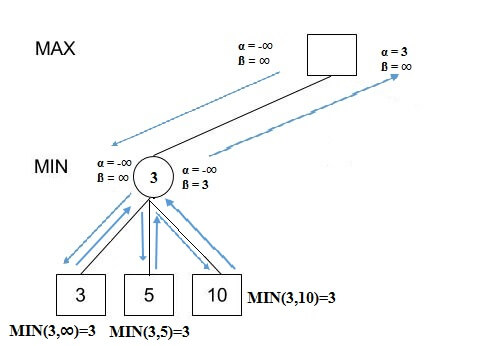
\includegraphics[width=\textwidth]{images/ab}
                \end{figure}
            \end{frame}
                \begin{frame}
                    \frametitle{Alfa-Beta Pruning}
                    %https://en.wikipedia.org/wiki/Alpha–beta_pruning
                    %\begin{columns}
                    %    \column{0.4\textwidth}
                    %    \begin{figure}[H]
                    %        \centering
                    %        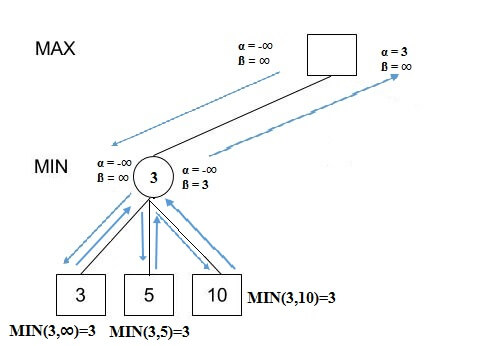
\includegraphics[width=\textwidth]{images/ab}
                    %        \caption{Działanie algorytmu}
                    %    \end{figure}
                    %    \column{0.6\textwidth}
                        \scalebox{0.7}{
                            \begin{minipage}{1.1\linewidth}
                        \begin{algorithm}[H]
                            \SetAlgoLined
                            \DontPrintSemicolon
                            \SetKwFunction{FMain}{alphabeta}
                            \SetKwProg{Fn}{Function}{:}{end}
                            \Fn{\FMain{node, depth, $\alpha$, $\beta$, maximizingPlayer}}{
                                \If{depth $=0$ or node is a terminal node}
                                {
                                    \KwRet heuristic value of node\;
                                }
                                \eIf{maximizingPlayer}
                                {
                                    value $\gets -\infty$\;
                                    \ForEach{child in node}{
                                    value $\gets$ max(value, alphabeta(child, depth $- 1$, $\alpha$, $\beta$, False))\;
                                    $\alpha \gets$ max($\alpha$, value)\;
                                    \lIf{$\alpha \geq \beta$}{break\;}
                                    }
                                    \KwRet value\;


                                }
                                {
                                    value $\gets +\infty$\;
                                    \ForEach{child in node}{
                                    value $\gets$ min(value, alphabeta(child, depth $- 1$, $\alpha$, $\beta$, True))\;
                                    $\beta \gets$ min($\beta$, value)\;
                                    \lIf{$\alpha \geq \beta$}{break\;}
                                    }
                                    \KwRet value\;

                                }
                            }
                            \;
                        \end{algorithm}
                    \end{minipage}
                    }
                    %\end{columns}
                \end{frame}
            
            \subsubsection{Monte Carlo tree search}
                \begin{frame}
                    \frametitle{Monte Carlo tree search}
                    %https://en.wikipedia.org/wiki/Monte_Carlo_tree_search
                    \begin{itemize}
                        \item<1-> Selekcja - Wybór liścia w drzewie gry
                        \item<2-> Ekspansja - Utworzenie węzła potomnego - jeżeli liść nie kończy gry
                        \item<3-> Symulacja - rozegranie losowej gry z wybranego węzła
                        \item<4-> Propagacja wsteczna - aktualizacja informacji w węzłach na podstawie wyniku rozegranej gry                         
                    \end{itemize}
                    
                    \begin{figure}[H]
                        \centering
                        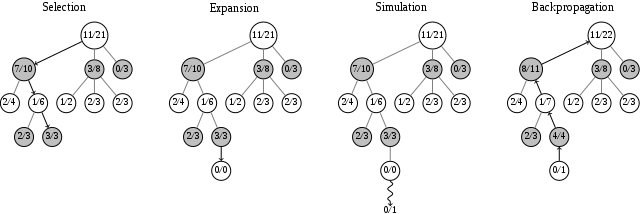
\includegraphics[width=0.9\textwidth]{images/mcts}
                        \caption{Monte Carlo tree search}
                    \end{figure}
                    
                \end{frame}
            \subsubsection{Null move}
            \begin{frame}
                \frametitle{Null move}
                %https://en.wikipedia.org/wiki/Killer_heuristic
                \begin{itemize}
                    \item<1-> Ruch zerowy, czyli pasowanie
                    \item<2-> W szachach jest niedozwolony
                    \item<3-> Założenie: zrzeczenie się ruchu jest gorsze niż wykonanie dowolnego legalnego ruchu
                    \item<4-> Wykorzystywane w poszukiwaniu zagrożeń
                    \item<5-> Może powodować błędy np. będąc szachu
                \end{itemize}
                %na koniec
                %heurystyka ruchu zerowego null move, jako przyklad tylko
            \end{frame}
            \subsubsection{Killer heuristic}
                \begin{frame}
                    \frametitle{Killer heuristic}
                    \begin{itemize}
                        \item<1-> Autorka: Barbara Liskov
                        \item<2-> Tylko niewielka liczba ruchów diametralnie zmienia sytuację
                        \item<3-> Założenie: jeżeli ruch tworzy odcięcie \textit{(zabójczy ruch)}, to prawdopodobnie wytworzy je też w podobnej sytuacji
                        \item<4-> Aby przyśpieszyć odcięcie algorytm rozpoczyna szukanie od zapisanych \textit{zabójczych ruchów}
                    \end{itemize}
                    %https://en.wikipedia.org/wiki/Killer_heuristic
                    %na koniec
                    %heurystyka ruchu zerowego null move, jako przyklad tylko
                \end{frame}
            
    \section{Literatura}
        \begin{frame}
            \frametitle{Literatura}
            \scalebox{0.7}{
                            \begin{minipage}{1.3\linewidth}
            \begin{thebibliography}{9}
                \bibitem{tictactoe}Anurag Bhatt, Pratul Varshney, Kalyanmoy Deb, Indian Institute of Technology Kanpur, \emph{Evolution of No-loss Strategies for the Game of Tic-Tac-Toe}, \url{https://www.iitk.ac.in/kangal/papers/k2007002.pdf} (data dostępu: 28.10.2019)
                \bibitem{course_gt}Martin J. Osborne, Ariel Rubinstein, The MIT Press, \emph{A course in Game Theory}, 1994
                \bibitem{ai_history}Andrey Kurenkov, \emph{A 'Brief' History of Game AI Up To AlphaGo}, \url{https://www.andreykurenkov.com/writing/ai/a-brief-history-of-game-ai/} (data dostępu: 26.10.2019)
                \bibitem{wiki_solved_game}Wikipedia, \emph{Solved game}, \url{https://en.wikipedia.org/wiki/Solved_game} (data dostępu: 26.10.2019)
                \bibitem{minichess}Mehdi Mhalla, Fr\'ed\'eric Prost, \emph{Gardner’s Minichess Variant is solved}, \url{https://arxiv.org/pdf/1307.7118.pdf} (data dostępu: 27.10.2019)
                \bibitem{hex_proof} \emph{Hex}, SP.269, Spring 2011 \url{http://web.mit.edu/sp.268/www/hex-notes.pdf} (data dostępu 03.11.2019)
            \end{thebibliography}
        \end{minipage}
            }
        \end{frame}
\end{document}